\documentclass[conference]{IEEEtran}
\IEEEoverridecommandlockouts
% The preceding line is only needed to identify funding in the first footnote. If that is unneeded, please comment it out.
\usepackage{cite}
\usepackage{amsmath,amssymb,amsfonts}
\usepackage{algorithmic}
\usepackage{graphicx}
\usepackage{textcomp}
\usepackage{xcolor}
\usepackage[export]{adjustbox}
\usepackage{algorithm}
\usepackage{float}
\usepackage{listings}
\def\BibTeX{{\rm B\kern-.05em{\sc i\kern-.025em b}\kern-.08em
    T\kern-.1667em\lower.7ex\hbox{E}\kern-.125emX}}

\usepackage{color}

\definecolor{mygreen}{rgb}{0,0.6,0}
\definecolor{mygray}{rgb}{0.5,0.5,0.5}
\definecolor{mymauve}{rgb}{0.58,0,0.82}

\lstset{ 
  backgroundcolor=\color{white},   % choose the background color; you must add \usepackage{color} or \usepackage{xcolor}; should come as last argument
  basicstyle=\footnotesize,        % the size of the fonts that are used for the code
  breakatwhitespace=false,         % sets if automatic breaks should only happen at whitespace
  breaklines=true,                 % sets automatic line breaking
  captionpos=b,                    % sets the caption-position to bottom
  commentstyle=\color{mygreen},    % comment style
  deletekeywords={...},            % if you want to delete keywords from the given language
  escapeinside={\%*}{*)},          % if you want to add LaTeX within your code
  extendedchars=true,              % lets you use non-ASCII characters; for 8-bits encodings only, does not work with UTF-8
  firstnumber=1000,                % start line enumeration with line 1000
  frame=single,	                   % adds a frame around the code
  keepspaces=true,                 % keeps spaces in text, useful for keeping indentation of code (possibly needs columns=flexible)
  keywordstyle=\color{blue},       % keyword style
  language=Octave,                 % the language of the code
  morekeywords={*,...},            % if you want to add more keywords to the set
  numbers=left,                    % where to put the line-numbers; possible values are (none, left, right)
  numbersep=5pt,                   % how far the line-numbers are from the code
  numberstyle=\tiny\color{mygray}, % the style that is used for the line-numbers
  rulecolor=\color{black},         % if not set, the frame-color may be changed on line-breaks within not-black text (e.g. comments (green here))
  showspaces=false,                % show spaces everywhere adding particular underscores; it overrides 'showstringspaces'
  showstringspaces=false,          % underline spaces within strings only
  showtabs=false,                  % show tabs within strings adding particular underscores
  stepnumber=2,                    % the step between two line-numbers. If it's 1, each line will be numbered
  stringstyle=\color{mymauve},     % string literal style
  tabsize=2,	                   % sets default tabsize to 2 spaces
  title=\lstname                   % show the filename of files included with \lstinputlisting; also try caption instead of title
}

\begin{document}

\title{Implementation of Dual-Purpose ADC/DAC Serial Peripheral Interface\\
{\footnotesize \textsuperscript{}
\thanks{Authors of this report can be reached at: willwu{@}wustl.edu, x.ye@wustl.edu}
}}

\author{\IEEEauthorblockN{Will Wu, Xueke Ye}
\IEEEauthorblockA{\textit{ESE-465: Digital Systems Laboratory} \\
\textit{Washington University in St. Louis}}}

\maketitle

\begin{abstract}
To equip our Microblaze\textregistered{} microcontroller with diverse signal processing capabilities, we need to interface with analog and digital signal converters. In this report, we present the design and implementation of a peripheral for the Microblaze \textregistered{} that utilizes the Serial Peripheral Interface (SPI) to communicate with signal converters. The peripheral we designed and implemented is dual-purpose, and therefore can be used to interface with both analog and digital signal converters.
\end{abstract}

\section{Introduction} \label{introduction}

Both analog and digital signals are widely used in the electronics industry. With their individual strength and weaknesses, analog and digital signals are each well-suited to transmit their subset of information. For example, analog signals possess higher information density, making them suitable to transmit video or audio signals. To receive and transmit both types of signals, conversion between analog and digital signals is required. 

Dedicated circuits have been designed to carry out such conversions. An Analog-to-Digital Converter (ADC) samples analog signals at a set sampling rate and transcribes the samples collected into digital signals. A Digital-to-Analog Converter (DAC) performs the reverse function. To the conversion capabilities of these devices, our Microblaze \textregistered{} Processor requires an interface to transmit/receive necessary signals to the external converters. 

Developed by Motorola, the Serial Peripheral Interface(SPI) \cite{b2} offers a robust time-synced bidirectional communication interface. In our case, building a SPI peripheral for the Microblaze\textregistered{} processor would allow it to interface with the signal converters. Hence, in this report, we present our design of a dual-purpose SPI peripheral for the Microblaze\textregistered{} that can both interface with ADCs and DACs. Our report is structured as follows: section \ref{design} outlines the logic design of the SPI peripheral; section \ref{testing} introduces testing methods as well as testing results, and section \ref{discussion} discusses the implication of our implementation.

\section{Design} \label{design}

The design of our SPI peripheral largely depends on the type of ADC and DAC we choose. In order to interface with both devices using a unified design, we need to take timing characteristics of both devices into account. We choose to interface with the \textit{LTC1865} ADC and the \textit{LTC1654} DAC, both manufactured by Analog Devices. Both devices offer SPI-compatible serial I/O for data transfer and device configuration. 
\paragraph{Timing}Consulting the device data sheets \cite{b3}\cite{b4}, we summarize the important timing requirements into the following table:

\begin{table}[htbp]
\caption{Important ADC and DAC Timing Constraints}
\begin{center}
\begin{tabular}{|c|c|c|c|}
\hline
\multicolumn{4}{|c|}{\textbf{Minimum and Maximum Timing Requirements}}\\
\hline
Label & Item & ADC & DAC\\
\hline
$t_1$ & $CONV/CS$ Setup time& $60ns$ (min) & $15ns$ (min)\\
\hline
$t_2$ & $SDI$ setup time& $15ns$ (min)& $45ns$ (min)\\
    &  before $SCK$ high & & \\
\hline
$t_3$ & $SDI$ hold time & $15ns$ (min) & $0ns$\\
    & after $SCK$ high  & & \\
\hline
$t_4$ & $SCK$ high time & $40\%$ $T_{SCK}$ & $20ns$ (min)\\
\hline
$t_5$ & $SCK$ low time & $40\%$ $T_{SCK}$ & $20ns$ (min)\\
\hline
$t_6$ & $CONV/CS$ low to & $120ns$ & N/A\\
    & valid $SDO$ delay & & \\
\hline
\end{tabular}
\label{software_timing}
\end{center}
\end{table}

Given the timing characteristics of both devies, we note that the ADC poses more timing restrictions than the DAC. Hence, we prioritize to accommodate for the ADC timing requirements in our SPI peripheral design. Given a set sampling rate of $25kHz$ and two channels for audio signal, we implement a "switch" sampling mode. The ADC will, in total, sample at $50kHz$, but it samples each channel alternatively. Consequently, signals from each channel are sampled at $25kHz$. 

Given the timing requirements of both devices, we design the SPI peripheral to generate the following timing signals (as shown in Fig~.\ref{timing}) in order to drive the ADC/DAC with correct timing. Note that the Microblaze\textregistered{} clock, $clk$, is also shown in the graph.

\begin{figure*}[htbp]
    \centerline{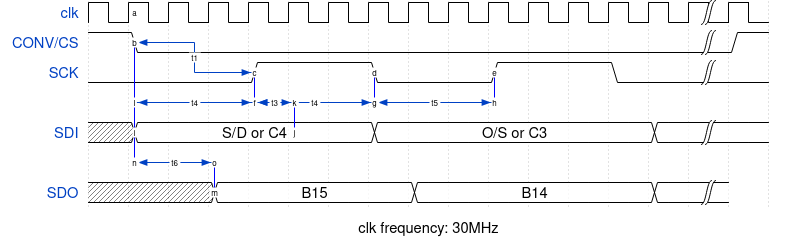
\includegraphics[width=\textwidth]{Figures/SPI/Screenshot from 2022-11-23 14-58-45.png}}
    \caption{SPI peripheral timing design}
    \label{timing}
\end{figure*}

\begin{figure*}[htbp]
    \centerline{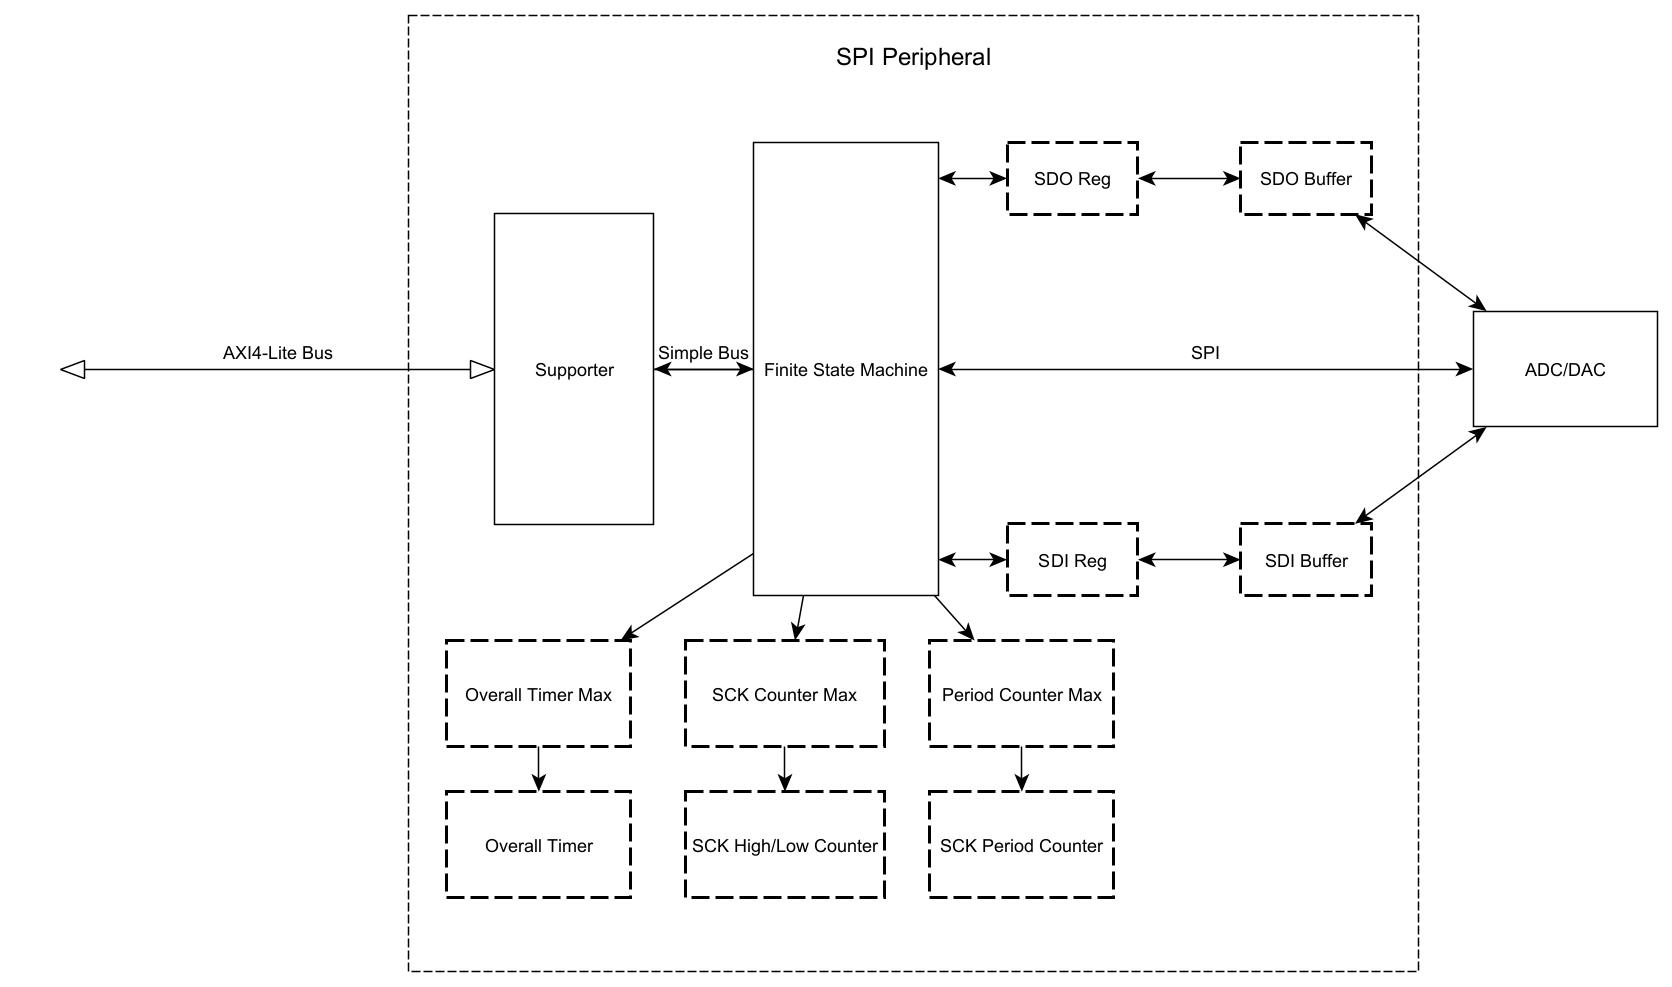
\includegraphics[width=\textwidth]{Figures/SPI/hardware_architecture.jpg}}
    \caption{Hardware architecture of the SPI peripheral}
    \label{hardware}
\end{figure*}

We have two important considerations regarding the timing design. First, all minimum setup and hold times must meet requirements even in the worse case scenarios. Second, even though DAC operations require lengthier SDI and SCK outputs, our SPI timing design still should meet the timing requirements for both. Given our timing design, we clearly meet the formal requirement: $SCK$ remains low for three $clk$ clock cycles after $CONV/CS$ goes low, satisfying the $30ns$ minimum set up time. Given that each $SCK$ cycle takes up $200ns$, and $CONV/CS$ must remain high for $3.2\mu{}s$, the timing design shown in Fig~.\ref{timing} still satisfies the sampling rate constraints, as shown by \eqref{adc_timing} and \eqref{dac_timing} below (given a $14ns$ delay):

\begin{equation}
    \text{ADC: }T_{total} = 3200 + 16\times 200 + 14 = 6414 < 10000(ns)
    \label{adc_timing}
\end{equation}

\begin{equation}
    \text{DAC: }T_{total} = 3200 + 21\times 200 + 14 = 8014 < 10000(ns)
    \label{dac_timing}
\end{equation}

\begin{figure*}[htbp]
    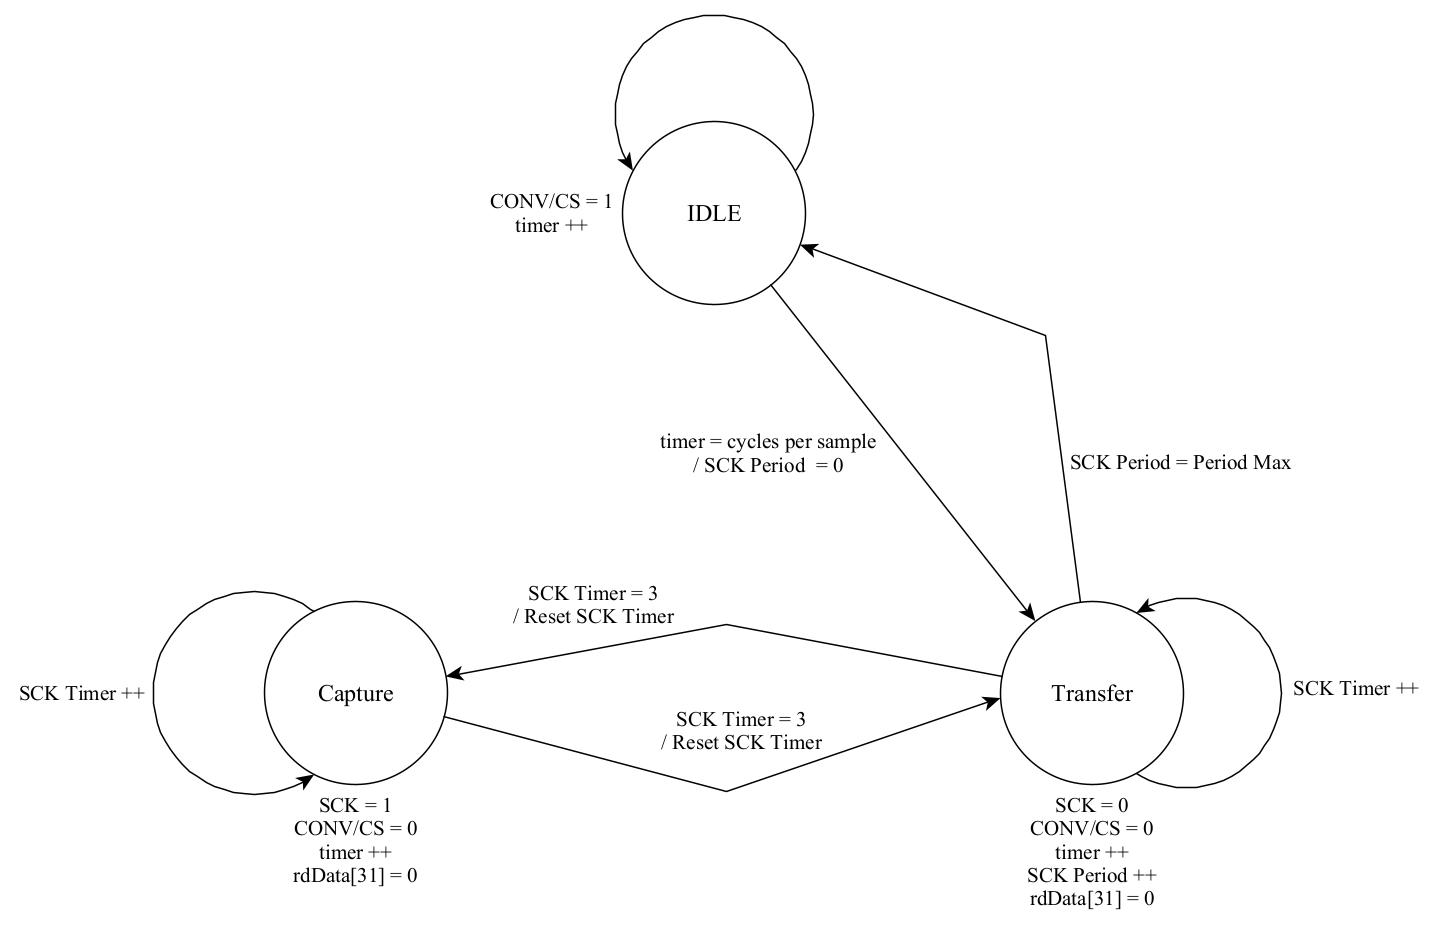
\includegraphics[width=1\linewidth, left]{Figures/SPI/timing.jpg}
    \caption{Illustration of the finite state machine}
    \label{fsm}
\end{figure*}

\paragraph{Logic} The time requirement design provides our peripheral with timing constraints. Similar to other projects, we aim to use a finite state machien to represent the internal logic of our peripheral. Unlike previous projects, however, the transition between logical states are now affected by timing. In other words, previous finite state machines we designed stay in the same state until certain logical conditions are met. For our SPI implementation, the finite state machine stays in the same state for a certain period of time, which is constrained by our timing design. Timing in hardware, in reality, poses little challenge to implement. Since the Microblaze \textregistered{} microcontroller runs on a set clock frequency, timing constraints can be represented as numbers of device clock periods. For example, since the Microblaze\textregistered{} runs at a clock frequency of $30MHz$, 3 complete clock cycles take up exactly $100ns$. 


The finite state machine of the peripheral, designed based on the timing diagram and the DAC/ADC operation sequence\cite{b3}\cite{b4}, is shown in Fig~.\ref{fsm}. A total of six timing registers, as shown in Fig~.\ref{hardware}, are tasked with timing the logical transitions used in the finite state machine that governs the SPI peripheral input/output signals. Three registers (that contain ``max'' in their labels) hold the period counts that represent the specific timing constraint, while the other three are used as counters. The timing constraint registers are modified by the Microblaze\textregistered{} processor, while the counter registers increase by 1 every clock cycle or by every $SCK$ cycle. When the counter registers hit the maximum value indicated by the timing constraint registers, the finite state machine, as a result triggers state transitions.

We also implemented four memory registers to store $SDI$ and $SDO$ data. Out of the four registers, two are ``buffer" memories while the rest are ``program" memories. The separation between program registers and buffer memories is necessary to prevent potential conflict between the peripheral and the signal converter. The peripheral only updates its buffer registers when $CONV/CS$ outputs high, which implies that the interfaced converter is not actively waiting for the $SDI$ input or actively outputting $SDO$.

\section{Operation and Testing} \label{testing}

\paragraph{Operation}The SPI peripheral is designed using Verilog, and implemented using a Xilinx Artix-7 FPGA, housed on a Digilent Nexys\texttrademark{} 4 DDR development board. We instantiate two SPI peripherals, one linked with the \textit{LTC1865} ADC and the other with the \textit{LTC1654} DAC. The peripherals are connected to the Microblaze\textregistered{} microprocessor with AXI4Lite buses.


\begin{figure*}[htbp]
    \centerline{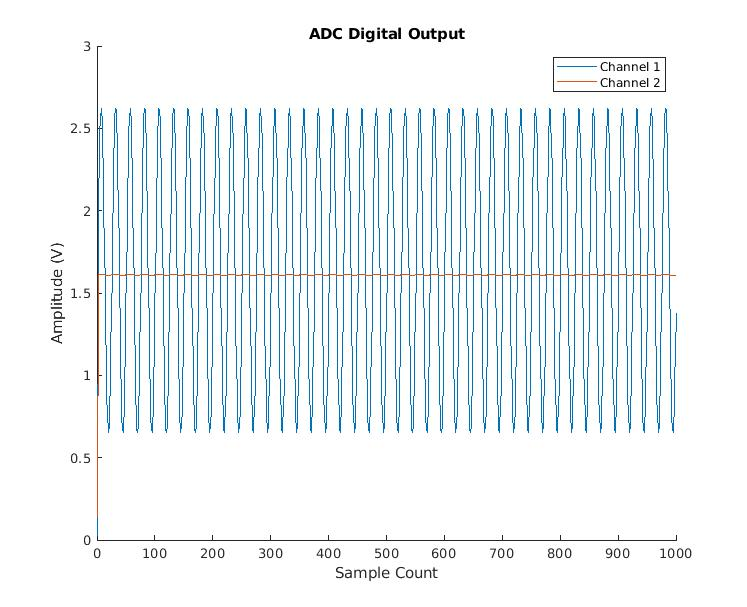
\includegraphics[width=0.7\textwidth]{Figures/SPI/ADC_out.jpg}}
    \caption{First 1000 ADC samples}
    \label{ADC_OUT}
\end{figure*}

We have written a C-program as the control program for the peripherals. The program serves three major functions. First, it configures the sampling frequency of the ADC/DAC peripheral by writing to the ``Overall Timer Max'' register. Given we sample at $50KHz$, and our clock runs at $30MHz$, we write in $600$ as the maximum clock cycles per sample. Second, it configures the total period of peripheral SCK signal based on the type of converter connected: our ADC in use requires roughly 16 periods of SCK, while our DAC in use requires 24. Third and foremost, the C-program serves as a read/write interface. It reads the converted digital signals from the ADC while writes digital signals to the DAC to be converted. Note that all read/write operations follow a polling model that ensures only one new data is read/written to the peripheral within 1 sampling period. As the SPI peripheral provides a confirmation bit (bit 32 in ``rdData") to indicate correct read/write timing, the program will continuously poll the peripheral for confirmation, but only reads/writes when it has confirmation. Serendipitously, the dual-purpose design of our SPI interface allows us to use only one control program. Additionally, it allows us to achieve a "loop-back mode", in which the program feeds sampled digital signals from the ADC into the DAC to replicate the original analog data. The source code to the C-program can be found in the appendix. 


\paragraph{Testing}Following the board bring-up process, we examine the SPI signals first to ensure correct peripheral operation. Using an oscilloscope, we can capture the digital SPI signals between our SPI pheripheral and the converters. Fig.~\ref{ADC_1} (in the appendix) shows the captured SPI signals connected to an ADC. Note that the two cursors measures the $CONV/CS$ setup time before first $SCK$ high. The setup time measures to $63.20ns$, which satisfies the minimum timing requirement of $30ns$. Fig.~\ref{ADC_2} subsequently shows correct channel switch during the ADC sampling cycle. Subsequent figures in the appendix, fig.~\ref{DAC_1} and fig.~\ref{DAC_2}, demonstrate correct SPI signals and thus correct SPI operation when connected to a DAC. 

ADC operations were tested first. Using a function generator, we feed in a sinusoidal signal with an amplitude of $1V$ and frequency of $1kHz$ into channel 1 of the ADC, while leaving channel 2 empty. We are expected to acquire a sine wave of the corresponding magnitude on channel 1, while a static signal on channel 2. Fig.~\ref{ADC_OUT} shows 1000 samples of the converted digital signal collected from channel 1 and channel 2. The signal frequency matches our expectation: $1kHz$. The signal magnitude of the sinusoidal signal also closely resembles the amplitude of the input signal: the samples yielded a peak-to-peak voltage of $2V$, which is equivalent to an amplitude of $1V$. Note that the magnitude of the output signals from channel 2 comes out to be $1.6V$, around half of the logical high voltage of the Nexys\texttrademark{} 4 DDR development board.

\begin{figure}[htbp]
    \centerline{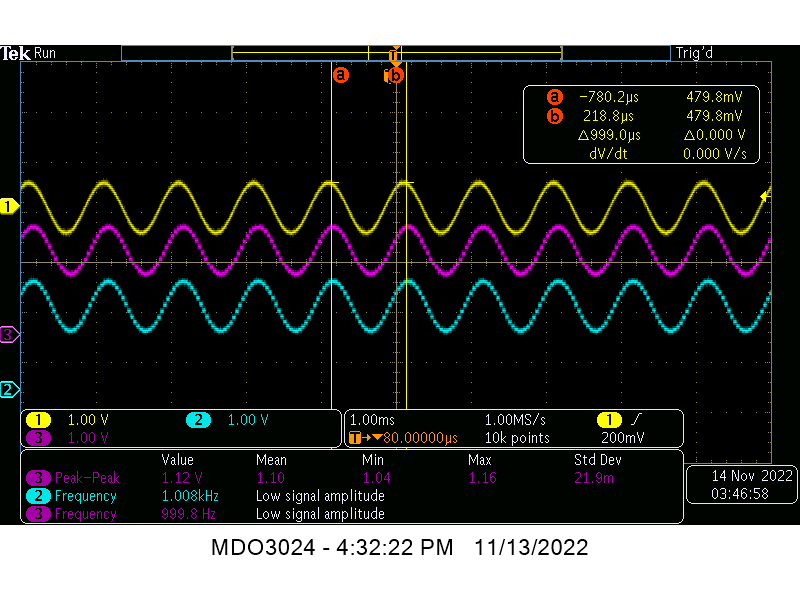
\includegraphics[width=\linewidth]{Figures/SPI/loop_back.png}}
    \caption{Loop back mode test result}
    \label{LOOP_BACK}
\end{figure}

DAC operations were subsequently tested by feeding a digital sinusoidal signal of 1000 samples into the SPI peripheral connected. The sinusoidal signal has an amplitude of $1V$ and frequency of $1kHz$. Using the "single trigger" mode on our mixed domain oscilloscope, we verify the correct operation of our DAC.

Lastly, continuous loop back mode is tested by simultaneously reading from both channels of the ADC and writing the converted digital signals to the ADC. We fed in a sinusoidal test signal of amplitude $1V$ and frequency $1kHz$ in both channels. Fig~.\ref{LOOP_BACK} shows the output signals (in blue and pink) from the DAC and the input reference (in yellow) into the ADC. We can consequently verify correct operation of the loop back mode.


\section{Discussion and Conclusion} \label{discussion}
This report presents the design, implementation and testing details of a dual-purpose SPI peripheral for the Microblaze\textregistered{} microprocessor. The peripheral can interface with both ADCs and DACs using the Serial Peripheral Interface. When instantiated correctly, the peripherals can operate in "loop-back" mode, where the output of the DAC replicates the input analog signal to the ADC. 

Combined with our previous digital FIR filter, we now can process analog signals digitally. The SPI peripherals, in loop-back mode, enable us to filter and output analog signals in real time. Digital signal output from the ADC can be fed into our previously designed FIR filters, which attenuate signals in undesirable frequency bands. The SPI peripherals enable us to interface with signal converters, thus providing us with a solid base to construct a real-time digital audio equalizer.

\begin{thebibliography}{00}
\bibitem{b1} P. Dahker, ``Introduction to SPI interface'', Analog Devices, 2018
\bibitem{b2} Motorola, Inc, ``SPI Block Guide V03.06'', 2003
\bibitem{b3} Analog Devices, Inc, ``LTC1864/LTC1865 Datasheet''
\bibitem{b4} Analog Devices, Inc, ``LTC1654 Datasheet''
\end{thebibliography}

\newpage
\onecolumn
For code and graphs, please see: 
\end{document}
